In an effort to help researchers glean insight from tweets, Twitter offers
a streaming API that streams all tweets that contain a certain string.
We leverage this service to gather data surrounding the popular television
show \textit{The Walking Dead} and then measure the number of tweets that occur each
hour over a time span.

Using the programming language Python and the library \texttt{tweepy}, a popular
wrapper for the Twitter streaming API, we collected all tweets containing the
hashtag ``\#thewalkingdead'' for three weeks from 2015-11-07 21:00 EST to
2015-11-23 21:00 EST. As this television show airs Sundays at 21:00 EST,
of particular importance is the tweets occurring around this time.
We therefore restrict our measurements to 24 hours prior to and 24 hours after
the television show's airing for the above three week time frame.

These measurements give rise to the time series presented in Figure \ref{tweets_plot}.
From this plot it is clear that, due to the weekly episodic nature of the television
show, there is a seasonal component to this time series. It also appears that
there is a trend component. Thus, in order to fit a stationary time series
to the underlying data, we will need to first apply transformations to the data.

\begin{figure}[!t]
  \centerline{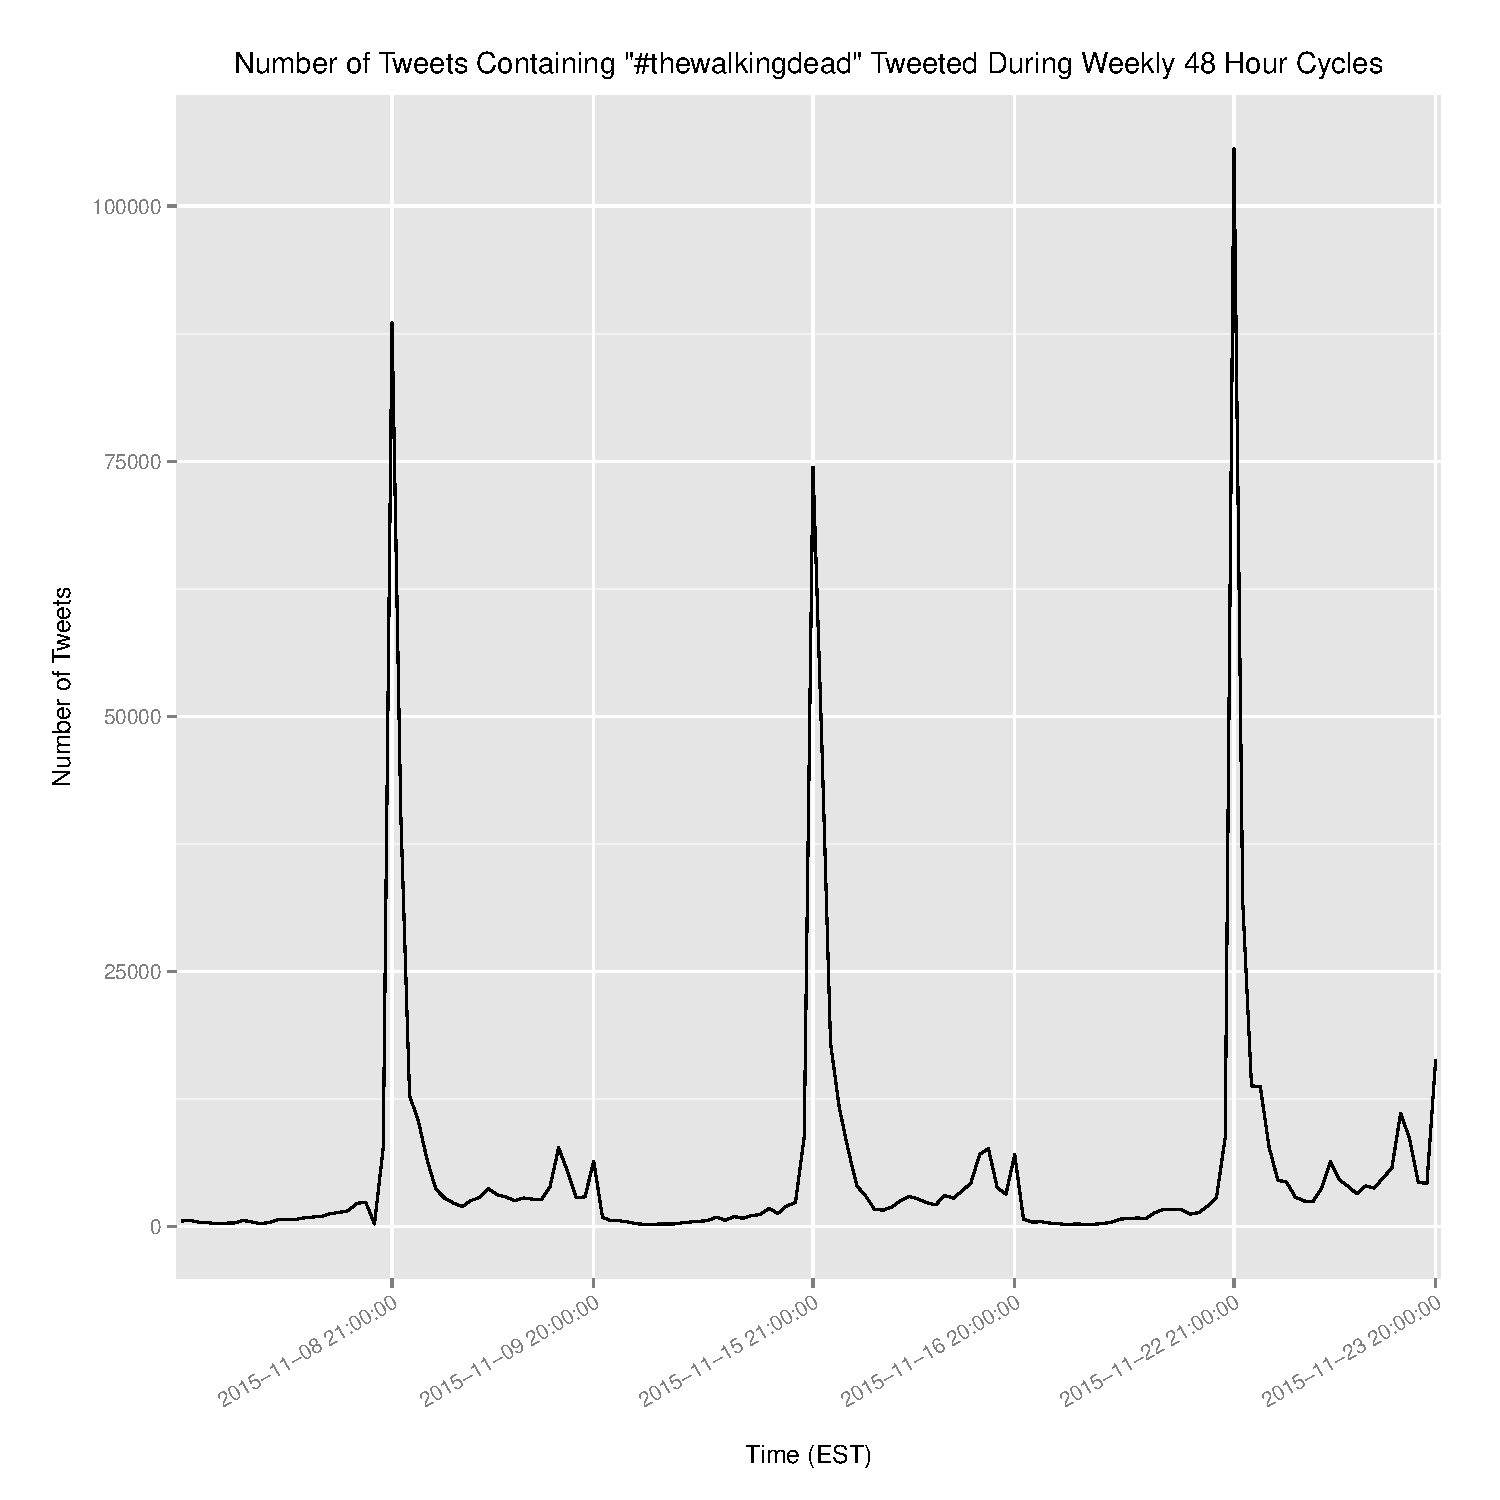
\includegraphics[scale=0.75]{../analysis/plots/tweets_plot}}
  \caption{Time series plot of number of tweets containing the hashtag
  \#thewalkingdead over three 48 hour cycles.}\label{tweets_plot}
\end{figure}

The details behind the process of fitting a stationary time series model to this data is handled in
Section \ref{model}.